\documentclass{beamer}
\usepackage{graphicx}
\usepackage{multicol}
\usepackage{vwcol}
\usepackage{bm}

%\usepackage{enumitem}
%\setlistdepth{9}
%\setitemize{label=\usebeamerfont*{itemize item}%
%  \usebeamercolor[fg]{itemize item}
%  \usebeamertemplate{itemize item}}

\title{Elliptic Curve Digital Signature Algorithm}
\author{Kevin Linger and Palmer Dabbelt}
\date{December 13, 2013}

\begin{document}
\maketitle

\begin{frame}
  \frametitle{Public Key Cryptography}


  \begin{itemize}
  \item Two keys (called a keypair)
    \begin{itemize}
    \item Public: the whole world can know this
    \item Private: only the owner knows this
    \end{itemize}
  \item Four operations
    \begin{itemize}
    \item \texttt{Sign(Message, Private)} $\rightarrow$ \texttt{Signature}
    \item \texttt{Verify(Message, Signature, Public}) $\rightarrow$ \texttt{Boolean}
    \item \texttt{Encrypt(Message, Public)} $\rightarrow$ \texttt{Cyphertext}
    \item \texttt{Decrypt(Cyphertext, Private}) $\rightarrow$ \texttt{Message}
    \end{itemize}
  \item ECDSA is a widely-used (SSH, SSL/TLS) signature algorithm
    \begin{itemize}
    \item Supports \texttt{Sign} and \texttt{Verify}
    \end{itemize}
  \end{itemize}
\end{frame}

\begin{frame}
  \frametitle{Cryptography and the Swarm}

  \begin{itemize}
  \item Original motivation: the universal dataplane
    \begin{itemize}
      \item Large network ($10^{10}$ nodes)
      \item Many low power sensors ($\bm{\mu} \mathbf{W}$)
      \item Some high power servers
    \end{itemize}
  \item Goal: all storage is fault-tolerant
    \begin{itemize}
    \item Byzantine fault tolerence algorithm
    \item Sign every message on the sensors
    \end{itemize}
  \item Problem: ECDSA is $\mathbf{mJ}$ per signature!
  \end{itemize}
\end{frame}

\begin{frame}
  \frametitle{The Discrete Logarithm Problem}

  \begin{itemize}
  \item $b^k = g$
    \begin{itemize}
    \item Difficult in one direction (given $b$ and $g$ find $k$)
    \item Easy in another direction (given $b$ and $k$ find $g$)
    \end{itemize}
  \item Only asymetric for some groups
    \begin{itemize}
    \item $({\mathbb Z}_p)^\times$: Integers modulo some prime,
      repeating multiplication
    \item $GF(p)$: Elliptic curves modulo some prime, repeating
      addition
    \end{itemize}
  \item At the center of many public-key crypto schemes
  \end{itemize}
\end{frame}

\begin{frame}
  \frametitle{Elliptic Curve Cryptography}


  \begin{itemize}
  \item Elliptic curve: the set of points that satisfy
    $ y^2 = x^3 + ax + b $
    \begin{itemize}
    \item Need a finite field $\rightarrow$ everything's modular
    \item Needs to be difficult $\rightarrow$ modulo a large number
    \end{itemize}
  \item Add and multiply defined to satsify a field
    \begin{center}
      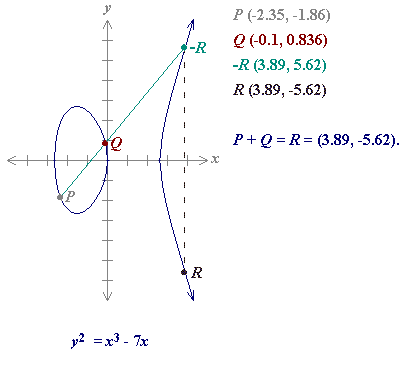
\includegraphics[width=0.6\linewidth]{point_add.png}
    \end{center}
  \end{itemize}
\end{frame}

\begin{frame}
  \frametitle{ECDSA}

  \begin{center}
    \begin{multicols}{2}
      \includegraphics[width=0.9\linewidth,height=0.7\textheight,keepaspectratio]{ecdsa_sign.uncrop.pdf} \\
      \includegraphics[width=0.9\linewidth,height=0.7\textheight,keepaspectratio]{ecdsa_verify.uncrop.pdf} \\
    \end{multicols}
  \end{center}
\end{frame}

\begin{frame}
  \frametitle{Point Operations}

  \begin{itemize}
  \item ECDSA is essentially point multiply and some cleanup
    \begin{itemize}
    \item Point Multiply: O(million) cycles
    \item Cleanup: O(thousand) cycles
    \end{itemize}
  \item Point multiplication is defined as repeated point doubling
  \item Point doubling is defined as
    $$ \left(\frac{(3 P_x^2 + a)}{(2 P_y)} - P_x \right)^2 * \left(\frac{(3 P_x^2 + a)}{(2 P_y)}\right) - P_y$$
  \item Simplifies to 5 modular multiplies and one modular divide
    \begin{itemize}
    \item Modular operations are modulo a large (O(256-bit)) number
    \end{itemize}
  \end{itemize}
\end{frame}

\begin{frame}[fragile]
  \frametitle{The Design Space}

  \begin{itemize}
  \item A whole bunch of math
    \begin{itemize}
    \item Data types: Points, Modular integers, and integers
    \item Arithmatic operations: Add, Subtract, Multiply, Invert
    \end{itemize}
  \item Everything boils down to integer arithmetic and control logic
    \begin{itemize}
    \item What should be in software, what should be in hardware?
    \end{itemize}
  \item Unfortunately, it's too big!
    \begin{itemize}
    \item $2^{12}$ software configurations!
    \end{itemize}
  \end{itemize}
\end{frame}

\begin{frame}[fragile]
  \frametitle{Hardware-Software Cotuning}

  \begin{itemize}
  \item OpenSSL is the industry standard, but it's difficult to hack on
  \item Wrote our own ECDSA implementation in C++
  \item Generates software for a family of ECDSA accelerators
  \end{itemize}

\begin{center}
\begin{minipage}{0.65\linewidth}
\tiny
\begin{verbatim}
palmer palmer-caldesktop rocket-ecc $ time make check | tail -n0
real    12m1.390s
user    63m20.796s
sys     7m37.179s
\end{verbatim}
\begin{verbatim}
palmer palmer-caldesktop rocket-ecc $ ptest | tail -n4
NRUN    6895
NPASS   6895
NFAIL   0
NEROR   0
\end{verbatim}
\end{minipage}
\end{center}

\end{frame}

\begin{frame}
  \frametitle{The (Reduced) Design Space}

  \begin{multicols}{2}
    \begin{minipage}{\linewidth}
      Point Multiplication
      \begin{itemize}
      \item Control logic
      \item Point Addition
        \begin{itemize}
        \item Control logic
        \item Modular multiply
          \begin{itemize}
          \item Control logic
          \item Integer shifts, adds
          \end{itemize}
        \item Modular inverse
          \begin{itemize}
          \item Control logic
          \item Integer shifts, adds
          \end{itemize}
        \end{itemize}
      \end{itemize}
    \end{minipage}

    \begin{minipage}{\linewidth}
      \begin{itemize}
      \item Two interesting hardware configurations
        \begin{itemize}
        \item Point multiply hardware block
        \item Modular multiply, inverse hardware blocks
        \end{itemize}
      \end{itemize}
    \end{minipage}
  \end{multicols}
\end{frame}

\begin{frame}
  \frametitle{Our Rocket Coprocessor}

  \begin{center}
    \begin{minipage}{0.5\linewidth}
      \input{rocket_coproc-small.svgtex}
    \end{minipage}
  \end{center}
\end{frame}

\begin{frame}
  \frametitle{Results}

  \begin{center}
    \begin{tabular}{c|ccc}
      Platform        & Power & Speed  & Area \\
                      & mJ/op & op/sec & mm$^2$ \\
      \hline
      OpenSSL (45nm)  & 20    & 1000   &      \\
      x86 (45 nm)     & 4000  & 5      &      \\
      Rocket          & 800   & 0.05   &      \\
      Virtex 2 (90nm) & 4000  & 250    &      \\
      Virtex 6 (45nm) & 500   & 4000   &      \\
      \hline
      Mod Mul         & 200   & 0.3    & 0.04 \\
      Mod Mul+Div     & 2     & 20     & 0.10 \\
      Point Add       & 0.5   & 100    & 0.31 \\
      Point Mul       & 0.06  & 400    & 0.35 \\
    \end{tabular}
  \end{center}
\end{frame}

\begin{frame}
  \frametitle{Future Work}

  \begin{itemize}
  \item Time-space tradeoffs
    \begin{itemize}
    \item Montgomery multipliers
    \item Projective point representation
    \end{itemize}
  \item Parallel software, multiple signatures in flight
  \item Hard-coded curve parameters
  \item 300MHz clock
  \end{itemize}
\end{frame}

\end{document}
